
\documentclass[11pt,titlepage,a4paper]{report}

%INCLUSIONE PACCHETTI
%---------------------------------------------
\usepackage[italian]{babel}
\usepackage{fancyhdr}
\usepackage{graphicx}
\graphicspath{{./pics/}} % cartella di salvataggio immagini

% STILE DI PAGINA
%---------------------------------------------
\pagestyle{fancy}
\renewcommand{\sectionmark}[1]{\markright{\thesection.\ #1}}
\lhead{\nouppercase{\rightmark}}
\rhead{\nouppercase{\leftmark}}
\renewcommand{\chaptermark}[1]{%
\markboth{\thechapter.\ #1}{}}

%Ridefinisco lo stile plain della pagina
\fancypagestyle{plain}{%
	\lhead{
\includegraphics[height=50pt]{logo.eps}}
	\chead{}
	\rhead{HappyCode inc \\ happycodeinc@gmail.com}
	\lfoot{BR-jsys}
	\cfoot{\thepage}
	\renewcommand{\headrulewidth}{1pt}
	\renewcommand{\footrulewidth}{1pt}
}
% layout
\begin{document}
%definizione variabili 
\newcommand{\lv}{ 0.3 } % latest version
\newcommand{\Glossario}{} %latest version
\newcommand{\dt}{ Manuale Utente }% Document title
\newcommand{\Grammatica}{}} % paragrafo dove si trova la spiegazione della grammatica
%common variables
\newcommand{\br}{\underline{business rule}}
\newcommand{\brs}{\underline{business rules}}
\newcommand{\bo}{\underline{business object}}
\newcommand{\bos}{\underline{business objects}}
\newcommand{\rp}{\underline{repository}}
\newcommand{\brp}{BusinessRuleParser}
\newcommand{\brl}{BusinessRuleLexer}
\newcommand{\BR}{\underline{BusinessRule}}

%nomi dei componenti
\newcommand{\AT}{Alessia Trivellato}
\newcommand{\ET}{Elena Trivellato}
\newcommand{\FC}{Filippo Carraro}
\newcommand{\LA}{Luca Appon}
\newcommand{\MB}{Michele Bortolato}
\newcommand{\MT}{Marco Tessarotto}
\newcommand{\MM}{Mattia Meroi}%altre variabili
% ultime versioni dei documenti da modificare solo alla fine
\newcommand{\AR}{AnalisiDeiRequisiti.2.6.pdf}
\newcommand{\DdP}{DefinizioneDiProdotto.0.9.pdf}
\newcommand{\G}{ Glossario.1.8.pdf }
\newcommand{\NdP}{NormeDiProgetto.2.0.pdf}
\newcommand{\PdQ}{ PianoDiQualifica.2.0.pdf }
\newcommand{\PdP}{ PianoDiProgetto.1.7.pdf }
\newcommand{\ST}{SpecificaTecnica.1.5.pdf}
\newcommand{\TR}{TestReport.0.7.pdf}
\newcommand{\MU}{ManualeUtente.0.3.pdf}%nomi documenti
%fine definizione variabili
\hyphenation{
 a-na-lo-go
 as-so-cia-zio-ne
 %attività non si può inserire come tutte le parole accentate che vanno messe nel testo semplice scritte at\-ti\-vi\-tà o come variabile
 coe-ren-za
 com-po-nen-ti
 des-crit-te
 des-cri-zio-ni
 di-a-gram-ma
 di-a-gram-mi
 e-le-men-to
 e-se-gui-re
 e-si-sten-ti
 es-pli-ci-to
 glo-bal-men-te
 glos-sa-rio
 li-vel-lo
 ne-ces-sa-rio
 per-met-te-re
 re-po-si-to-ry
 re-vi-sio-na-men-to
 ri-chies-te
 se-gna-la-ta
 va-li-da-zio-ne
 va-ria-bi-li
 ve-ri-fi-ca-re
 vi-sua-liz-za-te
 e-ven-tua-li
 o-pe-ra-zio-ne
 ar-chi-via-zio-ne
 mo-di-fi-ca
}


%sillabazione
\begin{titlepage}
\begin{center}
\vspace*{0.5in}

\includegraphics{logo.eps}
\vspace*{0.2in}

{\Large \textbf{BR-jsys}}
{\Large \emph{business rules} per sistemi gestionali in architettura J2EE } 
\vspace{2in}

\Huge \textsc{ \dt }

\end{center}
\end{titlepage}
\vspace*{0.5in}%pagina del titolo

\begin{center}
\thispagestyle{plain}
\begin{table}[htbp]
\large{
\begin{tabular}{l}
\Large{\textbf{\textsf{Capitolato: ''BR-jsys``}}} \\
\begin{tabular}{||p{6cm}||p{6cm}||} \hline
\textbf{Data creazione:} & 2008/02/25 \\ \hline
\textbf{Versione:} & \\ \hline
\textbf{Stato del documento:} & Formale, esterno \\ \hline
% ----------------------------------------------------------------------------autori
\textbf{Redazione:} & \\ \hline
\textbf{Revisione:} & \\ \hline
\textbf{Approvazione:} & \\ \hline
\end{tabular} \\
\end{tabular}
}
\end{table}

\begin{table}[hbtp]
\large{
\begin{tabular}{l}
\Large{\textbf{\textsf{Lista di distribuzione}}} \\

\begin{tabular}{||p{6cm}||p{6cm}||} \hline
{HappyCode inc}& Gruppo di lavoro\\ \hline
{Tullio Vardanega, Renato Conte}& Rappresentanti del committente \\ \hline
{Zucchetti S.r.l}& Azienda committente\\ \hline
\end{tabular} \\
\end{tabular}
}
\end{table}
\begin{table}[hbtp]
\large{
\begin{tabular}{l}
\Large{\textbf{\textsf{Diario delle modifiche}}} \\
\begin{tabular}{||p{2cm}||p{3.5cm}||p{6cm}||} \hline
%-------------------------------------------------------------------------------diario modifiche
\textbf{Versione} & \textbf{Data rilascio} & \textbf{Descrizione} \\ \hline
1.0 & 2008/03/04 & Inserimento sezione ``Azioni richieste/permesse'' \\ \hline
0.2 & 2008/03/01 & Completamento paragrafo ``Istruzioni per l'uso'' \\ \hline
0.1 & 2008/02/25 & Stesura preliminare del documento \\ \hline

\end{tabular} \\
\end{tabular}

}
\end{table}
\end{center}
\newpage

\tableofcontents 

\chapter{Introduzione}
Il presente documento contiene la definizione dell'architettura logica del sistema ``BR-jsys'' con una descrizione pi\`u accurata di ogni singola componente.
\section{Definizione dell'utente del prodotto}
Il prodotto \`e rivolto ad un utente al quale non sono richieste particolari conoscenze nel campo informatico. A tale scopo il software mette a dispozione:
\begin{itemize}
\item un'interfaccia grafica user-friendly;
\item messaggi di testo che aiutano l'utente dando informazione aggiuntive sullo stato del prodotto ``BR-jsys''.
\end{itemize}
\section{Come leggere il manuale}
Questo manuale presenta il sistema ``BR-jsys'' da noi realizzato e insegna come usare tutte le funzioni ad esso correlate. \`E organizzato in tre sezioni in modo da rendere facile il reperimento delle informazioni desiderate:
\begin{itemize}
\item SEZIONE GENERALE: dedicata alla descrizione generale del prodotto. Fornisce informazioni di base sul funzionamento del prodotto.
\item SEZIONE DETTAGLIATA: dedicata alla descrizione dettagliata. Indispensabile per un corretto utilizzo di ogni singola parte del prodotto.
\item SEZIONE APPENDICE: riporta gli errori pi\`u comuni che l'utente pu\`o riscontrare durante l'utilizzo del prodotto e il glossario per chiarire la terminologia da noi adottata.
\end{itemize}
Verranno riportati quindi tutti i passi che si possono effettuare, grazie anche all'ausilio di immagini dell'applicazione.
\section{Documenti utili}
Il presente manuale descrive totalmente il sistema e non richiede la lettura di ulteriori documenti. Tuttavia ogni utente deve avere installato nel proprio pc ``eXist'' in quanto vero e proprio requisito di sistema. 
\section{Come riportare problemi e malfunzionamenti}
Il prodotto software \`e dotato di un sistema di archiviazione svn. Tale archivio fornisce una sezione ``issues'' all'URL: \\ 
\textbf{``http://code.google.com/p/br-jsys/issues/list''}, che visualizza in qualsiasi momento la lista aggiornata di tutti i problemi e malfunzionamenti da noi riscontrati. Attraverso questo sistema ogni componente del gruppo potr\`a creare un ``new issue'', assegnandogli una priorit\`a che varier\`a a seconda della gravit\`a del problema. Ogni issue conterr\`a inoltre il nome dell'utente che lo ha aggiunto nella lista, oltre ad uno status (new, accepted, started, verified, etc...) che in qualsiasi momento ogni membro del gruppo potr\`a aggiornare. 

\chapter{Descrizione generale}
Il prodotto BR-jsys permette di testare la consistenza di business objects. A tale scopo il software mette a disposozione, attraverso la propria interfaccia grafica, la possibilità di inserirmento di business rules validate, cancellazione e querying nel repository.


\section{Caratteristiche del servizio}
% da fare

\section{Requisiti minimi}
\subsection{Requisiti sofware}
Sistema operativo:
\begin{itemize}
\item Linux: tutte le piattaforme con qualsiasi distribuzione.
\item Windows: WindowsME, Windows2000 e WindowsXp home/professional.
\item MacOSX: 10.4
\item eXist 1.2
\end{itemize}
Per usufruire del servizio \`e necessario possedere una connessione con il DBMS ``eXist'', come gi\`a citato precedentemente e la presenza della Java SE Development Kit (JDK) dalla versione 1.4.
\subsection{Requisiti hardware}
Per un corretto e scorrevole funzionamento del software sono richiesti:
\begin{itemize}
\item Processore 850Mhz.
\item 128Mb Ram.
\item 1Mb di spazio libero su disco.
\end{itemize}

\chapter{Istruzioni per l'uso}
\section{Descrizione funzionale}
Di seguito \`e riportata la descrizione delle funzioni del prodotto. Ad ogni passo \`e stata associata una figura, in modo da daterminare, senza amibiguit\`a il contesto dell'applicazione.
\subsection{Installazione}
Per utilizzare il prodotto \`e necessario che questo sia installato sulla macchina server. La sua architettura prevede che venga usato eXist, scaricabile liberamente al sito http://exist.sourceforge.net. Dopodich\`e:
\begin{itemize}
\item Linux e MacOSX: avviare il prompt dei comandi (shell), accedere alla cartella ``BR-jsys'' fornita e digitare il comando ``sh install''.
\item Windows: avviare il prompt dei comandi (shell), accedere alla cartella ``BR-jsys'' fornita e cliccare sulla sottocartella ``install.exe''.
\end{itemize}
\subsection{Avvio dell'applicazione}
Per avviare il programma una volta terminata l' installazione, sia in Linux che in Windows che in MacOSX, avviare il prompt dei comandi (shell), accedere alla cartella ``BR-jsys'' fornita e digitare ``BR-jsys.start''. Dopo un breve periodo di caricamento apparir\`a la schermata di login (figura 3.0), nella quale l' utente che accede per la prima volta al servizio dovr\`a digitare i dati: 
\begin{itemize}
\item username
\item password
\end{itemize}
\begin{figure}[htbp]
\begin{center}
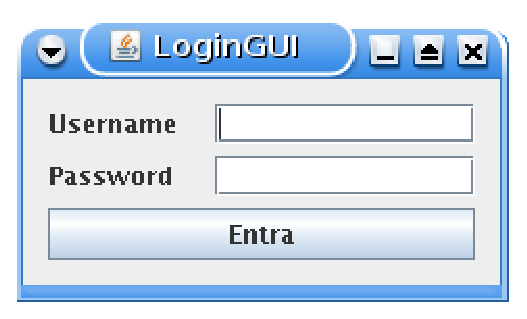
\includegraphics[width=0.4\textwidth]{manuale_utente/login.eps}
\end{center}
\caption{schermata di login}
\label{figura 3.0}
\end{figure}
I dati di autenticazione immessi sono quelli utilizzati per la registrazione al server ``eXist''. Tutti i dati richiesti dovranno essere insieriti prestando attenzione alla scelta della password, la quale dovr\`a avere una complessit\`a elevata. 

\section{Azioni richieste/permesse}
A questo punto verr\`a visualizzata la schermata principale (figura 3.1).
\begin{figure}[htbp]
\begin{center}
\includegraphics[width=0.4\textwidth]{manuale_utente/schermata_iniziale.eps}
\end{center}
\caption{schermata principale}
\label{figura 3.1}
\end{figure}
Nella figura 3.1 vediamo illustrate le tre funzionalit\`a associate ai rispettivi bottoni:
\begin{itemize}
\item Inserisci Business Rule;
\item Rimuovi Business Rule;
\item Sandbox.
\end{itemize}
L'analisi dettagliata delle singole azioni verr\`a trattata nelle sottosezioni seguenti.
\subsection{Inserisci Business Rule}
\begin{figure}[htbp]
\begin{center}
\includegraphics[width=0.4\textwidth]{manuale_utente/schermata_di_inserimento.eps}
\end{center}
\caption{schermata di inserimento}
\label{figura 3.3}
\end{figure}
Nella figura 3.3 vediamo illustrata la schermata di inserimento di una nuova business rule. L'utente dovr\`a inserire negli appositi spazi i campi dati richiesti:
\begin{itemize}
\item Nome: il nome della business rule che l'utente intende inserire (il nome dovr\`a essere significativo)
\item BO Associato: il nome della classe del business object alla quale si vuole associare la regola.
\item Regola: la regola scritta secondo la grammatica spiegata nel paragrafo \Grammatica.
\item Commento: descrizione sintetica del comportamento della regola. 
\end{itemize}
L'utente dovr\`a ora cliccare su ``Valida''. Se l'inserimento viene effettuato con successo verr\`a visualizzato un messaggio che ne conferma l'esito positivo, in caso contrario uno negativo.
\subsection{Rimuovi Business Rule}
\begin{figure}[htbp]
\begin{center}
\includegraphics[width=0.4\textwidth]{manuale_utente/schermata_di_rimozione.eps}
\end{center}
\caption{schermata di rimozione}
\label{figura 3.4}
\end{figure}
Nella figura 3.4 vediamo illustrata la schermata di cancellazione di una business rule. L'utente dovr\`a inserire negli appositi spazi i campi dati richiesti:

\subsection{Sandbox}
\begin{figure}[htbp]
\begin{center}
\includegraphics[width=0.4\textwidth]{manuale_utente/schermata_della_sanbox.eps}
\end{center}
\caption{schermata della sanbox}
\label{figura 3.5}
\end{figure}
\section{Errori probabili e cause possibili}
% da fare{figura 3.0}
\end{figure}

\chapter{Appendice}
\section{Messaggi di errore e loro significato}
\begin{table}[htbp]
\begin{tabular}{||p{6.5cm}||p{6.5cm}||}
\hline
\textbf{Messaggio:} & \textbf{Descrizione:} \\ \hline
Oggetto associato \textless nome associato\textgreater\ inesistente! & Inserimento di una business rule con un business object associato non valido. \\ \hline
Campo dato \textless nome campo dato\textgreater\ non trovato: validazione interrotta! & Riferimento ad un campo dato sbagliato. La validazione viene interrotta. \\ \hline
Operazione non consentita! \textless tipo 1\textgreater\ != \textless tipo 2\textgreater\ : validazione interrotta! & Errore tra tipi. Esecuzione di un'operazione di confronto tra due tipi diversi. La validazione viene interrotta. \\ \hline
Errore sintattico \textless tutta la business rule scritta fino all'errore\textgreater\ : validazione interrotta! & Errore di scrittura nella business rule. La validazione viene interrotta. \\ \hline
Regola \textless nome regola\textgreater\  gi\`a presente: inserimento fallito! & La regola ha un nome gi\`a presente nel repository. Non verr\`a quindi inserita. \\ \hline
Collegarsi ad eXist! & Il server eXist non \`e avviato. \\ \hline
Dati di autenticazione non corretti! & Nome utente e/o password non inseriti correttamente. \\ \hline
\end{tabular} \\
\end{table}
\section{Glossario}
Viene fornito come documento esterno chiamato \Glossario.

\end{document}
